\documentclass[11pt]{standalone}
\usepackage{amssymb}
\usepackage{amsmath}
\usepackage[no-math]{fontspec}
\usepackage{unicode-math}
\setmainfont{Libertinus Sans}
\setsansfont{Libertinus Sans}
\setmathfont{Libertinus Math}
\usepackage{pgf,xcolor}
\usepackage{tikz}
\usetikzlibrary{arrows.meta, backgrounds, calc}
\usepackage{pgfplots}
\pgfplotsset{compat=newest}
\usepackage{pifont}

\definecolor{my_darkgray}{HTML}{484949}
\definecolor{my_lightgray}{HTML}{F3F4F4}
\definecolor{my_darkblue}{HTML}{005A94}
\definecolor{my_lightblue}{HTML}{CCDEE9}
\definecolor{my_yellow}{HTML}{FFEC7F}
\definecolor{my_red}{HTML}{E60000}
\definecolor{my_orange}{HTML}{E87846}

\begin{document}
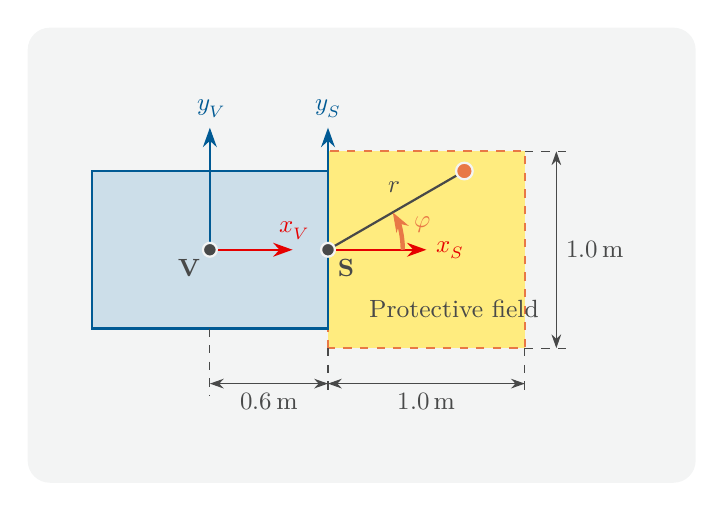
\begin{tikzpicture}[
    show background rectangle,
    background rectangle/.style={fill=my_lightgray, rounded corners=8pt},
    inner frame sep=0.8cm,
    achse/.style={thick, -{Stealth[length=7pt, width=5pt]}},
    bemassung/.style={draw=my_darkgray, thin, {Stealth[length=5pt, width=3.5pt]}-{Stealth[length=5pt, width=3.5pt]}},
    hilfslinie/.style={draw=my_darkgray, thin, dashed}
]

    % Draufsicht auf das FTF im Fahrzeugkoordinatensystem, Maßstab 1 m = 2.5 cm.
    % Fahrzeug 1.2 m x 0.8 m, Scanner in der Mitte der Vorderkante bei (0.6, 0),
    % Schutzfeld x_V von 0.6 bis 1.6 m, y_V von -0.5 bis 0.5 m.
    \coordinate (F) at (0,0);
    \coordinate (S) at (1.5,0);
    \coordinate (P) at ($(S)+(30:2.0)$);

    % Schutzfeld
    \draw[fill=my_yellow, draw=my_orange, thick, dashed] (1.5,-1.25) rectangle (4.0,1.25);
    \node[font=\small, text=my_darkgray] at (3.1,-0.75) {Protective field};

    % Fahrzeug: Umriss hellblau. Die Vorderkante ist hier nicht orange
    % hervorgehoben, weil die y_S-Achse auf ihr liegt.
    \draw[fill=my_lightblue, draw=my_darkblue, thick] (-1.5,-1.0) rectangle (1.5,1.0);

    % Fahrzeugkoordinatensystem F
    \draw[achse, draw=my_red] (F) -- (1.05,0)
        node[anchor=south, font=\small, text=my_red] {$x_V$};
    \draw[achse, draw=my_darkblue] (F) -- (0,1.55)
        node[anchor=south, font=\small, text=my_darkblue] {$y_V$};
    \node[font=\small\bfseries, text=my_darkgray, anchor=north east] at (F) {V};

    % Scannerkoordinatensystem S
    \draw[achse, draw=my_red] (S) -- (2.75,0)
        node[anchor=west, font=\small, text=my_red] {$x_S$};
    \draw[achse, draw=my_darkblue] (S) -- (1.5,1.55)
        node[anchor=south, font=\small, text=my_darkblue] {$y_S$};
    \node[font=\small\bfseries, text=my_darkgray, anchor=north west] at (S) {S};

    % Messstrahl mit Entfernung r und Winkel phi gegen die x_S-Achse
    \draw[draw=my_darkgray, thick] (S) -- (P);
    \node[font=\small, text=my_darkgray, anchor=south east] at ($(S)!0.6!(P)$) {$r$};
    \draw[draw=my_orange, ultra thick, -{Stealth[length=7pt, width=5pt]}]
        ($(S)+(0:0.95)$) arc[start angle=0, end angle=30, radius=0.95];
    \node[font=\small, text=my_orange] at ($(S)+(15:1.25)$) {$\varphi$};
    \draw[fill=my_orange, draw=my_lightgray, thick] (P) circle (3pt);

    % Ursprünge
    \draw[fill=my_darkgray, draw=my_lightgray, thick] (F) circle (2.5pt);
    \draw[fill=my_darkgray, draw=my_lightgray, thick] (S) circle (2.5pt);

    % Bemaßung in Fahrtrichtung
    \draw[hilfslinie] (0,-1.0) -- (0,-1.85);
    \draw[hilfslinie] (1.5,-1.25) -- (1.5,-1.85);
    \draw[hilfslinie] (4.0,-1.25) -- (4.0,-1.85);
    \draw[bemassung] (0,-1.7) -- (1.5,-1.7)
        node[midway, anchor=north, font=\small, text=my_darkgray] {$0.6\,\text{m}$};
    \draw[bemassung] (1.5,-1.7) -- (4.0,-1.7)
        node[midway, anchor=north, font=\small, text=my_darkgray] {$1.0\,\text{m}$};

    % Bemaßung quer zur Fahrtrichtung
    \draw[hilfslinie] (4.0,1.25) -- (4.55,1.25);
    \draw[hilfslinie] (4.0,-1.25) -- (4.55,-1.25);
    \draw[bemassung] (4.4,-1.25) -- (4.4,1.25)
        node[midway, anchor=west, font=\small, text=my_darkgray] {$1.0\,\text{m}$};

\end{tikzpicture}
\end{document}
